\chapter{O teste sistêmico na produção de placas de circuito impresso}
\label{rev}

%todo falar de PCOLA/SOQ/FAM do iNEMI (International Electronics Manufacturing Initiative)

Os testes de circuitos eletrônicos estão presentes em toda a cadeia de projeto, fabricação e operação de um produto. Sua relevância se nota desde as primeiras etapas de validação de um projeto de um sistema eletrônico, passando pelas etapas de produção de circuitos integrados, controle de qualidade do processo de montagem de placa, e até mesmo, no diagnóstico em campo do produto final. Como o presente trabalho discorre sobre testes de fim de linha de produção, o foco será nas etapas de teste finais na cadeia produtiva.

\section{Teste e diagnóstico pela cadeia produtiva: do circuito integrado ao teste sistêmico}

O teste de circuitos inicia-se no teste de circuitos integrados, na verificação de possíveis danos aos \textit{wafers} de silício. Em \citet{mitra2010post}, vê-se que estes testes se caracterizam pelo uso de jigas de teste complexas e uso de técnicas de projeto orientado à testabilidade (DfT) e, também, pela introdução de varredura periférica, autoteste embutido e compressão de dados de teste. 

Já na linha de montagem de placas de circuito impresso, existe variedade de abordagens possíveis para a realização de testes, medições e inspeções. Dentre as técnicas específicas desta etapa destacam-se a inserção de pontos de teste, inspeções óticas e de raio-x automatizadas, o uso de camas de prego nas jigas de teste e o uso do IEEE 1149.1, o JTAG. Cada uma dessas técnicas atendem objetivos específicos de teste e serão descritas nas próximas sessões ainda neste capítulo. Muitas vezes, a própria infraestrutura e funcionalidades de teste dos componentes integrados podem ser reutilizados no teste de placa, como no trabalho de \citet{cook2012reuse}, que descreve o reuso da infraestrutura de varredura periférica em testes em campo. 


% parte xyz
%aqui
Um esquema típico de uma linha de montagem de placas de circuito impresso é representado pela figura \ref{fig:linha}. Cada uma dessas categorias de teste tem por objetivo detectar um tipo específico de falha, de forma que juntos consigam atingir uma boa cobertura de teste. No trabalho de \citet{hird2002test}, o conceito de cobertura de teste é apresentado como a medida do quanto da placa de circuito impresso está verificada ou também como  um indicador numérico da qualidade do teste. Por ser uma medida de cobertura, há vários padrões de modelagem de cobertura de faltas. \citet{lotz2006functional} apresenta alguns padrões:

\begin{itemize}
    \item MPS (\textit{Material, Placement, Solder} - Material, Colocação e Solda), desenvolvido pela \textit{Philips Research};
    \item PPVS (\textit{Presence,  Polarity, Value, Solder} - Presença, Polaridade, Valor e Solda), desenvolvido pela  \textit{ASTER Ingénierie};
    \item PCOLA/SOQ  (\textit{Presence, Correctness, Orientation,  Live Alignment / Short, Opens, Quality} - Presença, Exatidão, Orientação, Vivo, Alinhamento / Curtos, Circuito Aberto, Qualidade), criado pela \textit{Agilent Technologies}, estende as métricas de teste para questões de interconexão;
    \item FAM (\textit{Feature, At-speed, Measurement} - Característica, em Velocidade Nominal, Medição) ou PCOLA/SOQ/FAM é uma extensão do item anterior. Foi desenvolvido pelo iNEMI para cobrir métricas funcionais  \citep{ley2009defect}.
    \item DMPSF (Design, Material, Placement, Solder, Function - Projeto, Material, Colocação, Solda, Função), desenvolvido por \citet{lotz2006functional}.
\end{itemize}

A partir de um destes padrões criam-se listas de controle para análise de cobertura de cada componente e interconexão da placa. Dessa forma, pode-se mensurar a cobertura de testes de um produto nos aspectos materiais, estruturais e funcionais.

\begin{figure}[ht]
    \centering
    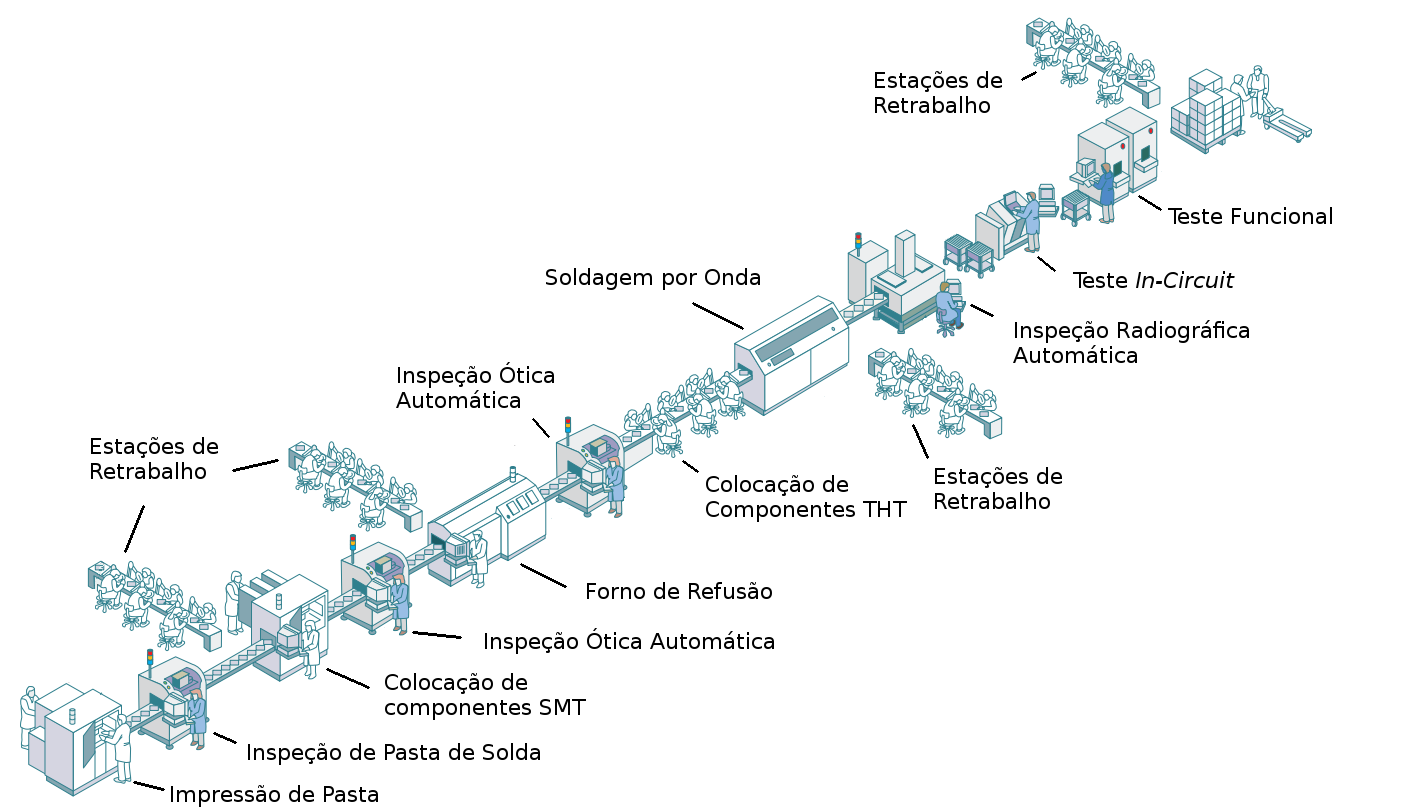
\includegraphics[width=1.1\linewidth]{linha.png}
    \caption{Uma típica linha de montagem de PCIs. Adaptado de \citet{agilenttechnologies2003}}
    \label{fig:linha}
\end{figure}


Juntamente com as métricas de cobertura de teste, os modelos de falta também cumprem um papel importante no estudo de testes de manufatura. \citet{jutman2014high} separa os modelos de falta nas seguintes classes: defeito materiais; defeitos em pinos e malha de circuito; problemas funcionais; e problemas de desempenho. 

Defeitos em materiais e mecânicos podem ser mensurados por métricas padrão de processo de qualidade e exemplificados por defeitos em placas, processo de montagem: solda ruim terminal levantado, componente defeituoso, desalinhamento, efeito lápide\footnote{Efeito Lápide, ou \textit{tumbstone effect}, é a elevação parcial ou total de componentes SMT passivos durante a refusão, assemelhando-se muitas vezes à uma lápide.}.

Os defeitos em pinos e malhas de circuito são modelados por análise estrutural e já possuem uma base bem estabelecida. Entram nessa classe as falhas de circuitos abertos ou em curto, defeito de driver (\textit{buffer}, pino).

Há ainda os problemas \textit{funcionais}, como falhas de \textit{boot}, cujas métricas são estabelecidas e investigadas por pesquisadores em desenvolvimento de software e lógica descritiva.
Por final, tem-se os problemas de desempenho em linhas de comunicação: alta taxa de erro, \textit{crosstalk, jitter, delay,} e outros.

Tradicionalmente na indústria, defeitos em materiais são solucionados durante a montagem da placa. Já os defeitos de pino, malha de circuito e funcional são testados no fim de linha de produção por duas categorias de teste denominados \textit{testes estruturais e testes funcionais}. A relação entre estas duas categorias de testes é descrita em  \citet{thomaswenzelenricozimmermann2016} e sintetizada na figura \ref{fig:cobertura}. Porém, em \citet{thomaswenzel2013} e \citet{jutman2014high}, nota-se que essa segmentação vem mudando com os avanços nas técnicas de verificação periférica e de teste centralizado por microcontrolador, que incorporam boa parte dos testes de desempenho e até mesmo funcionais. Tais técnicas serão descritas nas seção \ref{FCT} deste mesmo capítulo.

\begin{figure}[ht]
    \centering
    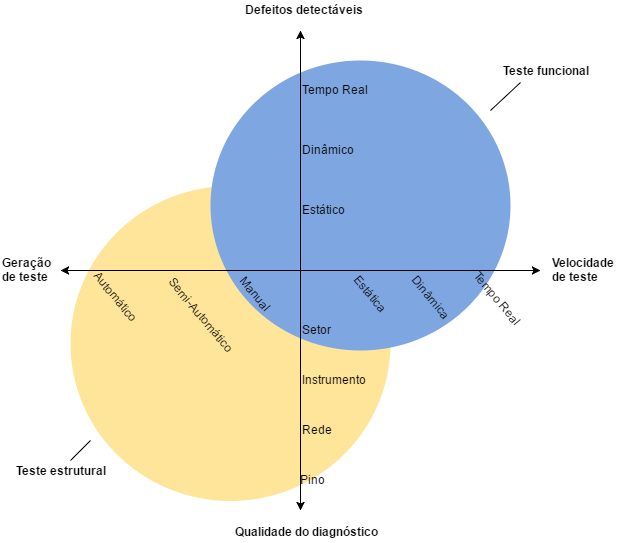
\includegraphics[width=1.0\linewidth]{complement.png}
    \caption{A complementariedade dos testes estruturais e funcionais para a cobertura de teste de um dispositivo. Adaptado de \cite{thomaswenzelenricozimmermann2016}.}
    \label{fig:cobertura}
\end{figure}

Viu-se aqui, portanto, que diversas técnicas e abordagens de teste e diagnóstico integram-se e são parte importante da produção, operação e manutenção de um sistema eletrônico. A seguir, estas técnicas serão descritas detalhadamente. 
\clearpage
\subsection{Inspeção de Pasta de Solda}

A inspeção de pasta de solda é o processo, normalmente automático, de achar falhas após a aplicação da pasta de solda. A inspeção de pasta de solda previne o retrabalho de placas com os componentes montados porque, uma vez com os erros de solda detectados, a placa defeituosa pode ser separada das demais. A detecção de falhas ainda nesta etapa custa 10 vezes menos do que uma falha pós refusão, ou após a solda, e 70 vezes menos que uma falha no teste elétrico intra-circuito (\textit{In-circuit test}) \citep{owen2000process}.

Os sistemas mais simples de inspeção de pasta de solda consistem de uma imagem colorida da placa. Este método consegue detectar ausência de solda e conexões indevidas entre blocos vizinhos, porém, por ser um método 2D, não consegue estimar a altura e volume da pasta de solda. Isso pode gerar problemas indetectáveis em outras etapas, já que, por mais que passe em testes de condutividade, a falta de pasta de solda em uma conexão pode causar problemas mecânicos e rompimento da interconexão. 

O volume de pasta de solda pode ser estimado por diversos métodos. \citet{5246351} introduz as principais tecnologias de perfilometria: 
\begin{itemize}
    \item Triangulação a laser;
    \item Perfilometria por fase, utilizando luz estruturada;
    \item Reconstrução por Redes Neurais.
\end{itemize}

Os métodos por triangulação a laser utilizam-se das projeções do feixe de laser no relevo da placa para reconstruir o seu perfil 3D.  \cite{5576321} descreve os detalhes desta técnica. Medições precisas podem ser obtidas com este método. Entretanto, são equipamentos caros, com baixa velocidade de inspeção, e susceptíveis a ruídos refletivos e \textit{efeito de sombras} \citep{5246351}.

Na perfilometria por fase, uma luz estruturada projeta um padrão, como uma grade ou uma série riscos, na PCI com a pasta de solda aplicada. Este padrão é então pouco a pouco deslocado e uma série de imagens são capturadas por uma câmera de alta resolução. Os sistemas mais avançados empregam um sistema livre de sombras onde ambos os lados da deposição de solda são caracterizados simultaneamente. \cite{5576321} oferece uma abordagem para o problema das sombras e \cite{5246351} faz uma revisão dos principais trabalhos em perfilometria por fase.

O método de reconstrução por redes neurais tenta resolver os problemas do \textit{shape-from-shading (SFS)}, que até então era um método cujo desempenho era inconsistente. \cite{5246351} revisa o estado da arte e propõe uma nova abordagem.

\subsection{Inspeção ótica automática - AOI}
% inserir https://repositorio.ufsc.br/xmlui/bitstream/handle/123456789/158843/337436.pdf?sequence=1&isAllowed=y

A inspeção ótica automática (AOI), como o próprio nome indica, inspeciona visualmente a placa de circuito por meio de fotos, processa e identifica automaticamente as falhas, seja de componente ou solda. Esta técnica é usada para detectar componentes trocados, faltantes ou mal posicionados e pode ser realizada na etapa pré-forno de refusão ou após, dependendo da particularidade do processo produtivo da fábrica. O trabalho de \cite{huang2015automated}, citado por \cite{mello2015sistema}, indica quatro categorias de inspeção ótica automática:

\begin{itemize}
    \item \textbf{Métodos de projeção}, que correlacionam a entrada com modelos aprendidos e suas características;
    \item \textbf{Abordagem baseada em filtro:} filtro espaciais com base em transformadas de sinal, como por exemplo, Fourier, Wavelet, discreta cosseno;
    \item \textbf{Aprendizagem de máquinas:} Os mais utilizados são as redes neurais, algoritmos genéticos, e máquinas de vetor suporte;
    \item \textbf{Abordagens híbridas:} associam diversas técnicas para classificações mais complexas. 
\end{itemize}

%A AOI na etapa pré-forno detecta componentes faltantes ou componentes errados, e alinhamento correto de componentes. Como este processo é realizado após a refusão, os defeitos são relativamente simples de corrigir e menos custosos do que após a etapa de refusão. Outra vantagem é que os problemas de calibração na máquina de posicionamento de componentes podem ser mais facilmente detectados e analisados. Uma análise de tendência nas etapas pós refusão não seria tão confiável, pois o processo de refusão altera a localização dos componentes, e problemas de calibração na máquina de posicionamento só seriam detectados após um aumento significativo de placas defeituosas.

%Na etapa pós refusão, a inspeção ótica automática é provavelmente a etapa mais aceita entre os fabricantes de placas eletrônicas. Um sistema AOI colocado nesta etapa detecta qualquer problema gerado ao longo do processo, incluindo defeitos de colocação de componentes e problemas relacionados à solda, como: falta ou excesso de solda, curto-circuitos ou circuitos abertos. Nesta etapa, a AOI detecta defeitos causados por problemas de impressão, pelo sistema de colocação de componentes, e ainda, pelo processo de refusão. O propósito da AOI após o processo de refusão não é somente prover dados de defeito necessários para o retrabalho de uma PCI, mas também para a coleta de dados através de múltiplas montagens de placa para análise de causa raíz e melhoramento contínuo da produção.

A maior limitação da AOI é a impossibilidade de detecção de defeitos em pinos ou partes do circuito não visíveis, como abaixo de componentes \textit{Ball Grid Array} (BGA) ou em circuitos eletromagneticamente blindados. Nesses casos, é necessário o uso de outras ferramentas, como a verificação de placas por radiografia.
%\cite{savage1993automated} citado por \citep{mello2015sistema}
%todo
\subsection{Inspeção radiográfica automática - AXI}

A inspeção radiográfica automática (AXI) possui uma vantagem única em relação às outras tecnologias de inspeção estrutural: os materiais absorvem os raios-x proporcionalmente à sua massa atômica. A solda utilizada na montagem das PCIs consiste de materiais pesados como o chumbo e a prata. A maioria restante dos materiais usados na fabricação das PCIs é composta por elementos leves como carbono, silício, alumínio, oxigênio, hidrogênio e cobre. Dessa forma, a inspeção radiográfica mostra-se muito interessante na geração de imagens do processo de solda: os pontos de solda aparecem muito bem, enquanto o restante da placa apresenta-se transparente. Outra vantagem é a possibilidade de inspecionar os pinos escondidos de encapsulamentos complexos como o BGA ou o \textit{chip-scale packages} (CSP), além de exibir características internas dos pontos de solda.

\subsubsection{Tipos de AXI}

 As técnicas AXI utilizadas em processos de manufatura e diagnóstico se dividem entre bidimensional e tridimensional \citep{7236817, dougmcclure2000}. 

A inspeção 2D é semelhante à radiografia convencional, porém com recursos de visão computacional para análise automática. É melhor aplicada em placas com soldas em um só lado da placa. Em placas com junções de solda em alta densidade ou em ambos os lados, a imagem gerada pode ficar confusa. 

Com a laminografia e tomografia computadorizada é possível obter a imagem de um recorte da placa e, associada a técnicas de processamento digital, reconstruir um modelo tridimensional da placa. A laminografia utiliza-se do movimento do emissor e detector que pode ser rotacional \citep{7236817} ou linear \citep{6756131}. A desvantagem da radiografia tridimensional é o tempo necessário para a captura da imagem e seu processamento \citep{6756131}. 

\subsubsection{Casos onde a inspeção radiográfica é importante}

\citet{leinbach2001and} apresenta três casos aonde a inspeção radiográfica se faz importante. Primeiro, na inspeção de componentes visualmente ocultos, como terminais de encapsulamentos CSP e BGA ou componentes sob blindagem RF. Segundo, em aplicações que exigem alta qualidade de solda, como as PCI expostas a ambientes de estresse mecânico ou térmico. Terceiro, em projetos de PCI complexos, cujas taxas de erro de produção por placa são mais frequentes e a AXI consegue garantir o rigor do processo de inspeção.

\citet{7236817} faz um estudo comparativo entre tecnologias de inspeção radiográfica para detecção de defeitos em furos galvanizados. \citet{7428398} aplicou AXI na inspeção de componentes \textit{press-fit} e \citet{7428400} na verificação do resinamento de placas de circuito impresso montadas. Combinada com técnicas de ICT, a maior parte dos defeitos podem ser cobertos. O trabalho de \citet{oresjo2002use} comenta melhor a relação entre AOI, AXI, e os testadores intra-circuito (\textit{in-circuit testers - ICT}).

\subsection{Testes intra-circuito (\textit{In-Circuit Testers - ICT)}}

Jigas de teste são uma grande ferramenta de teste de placas de circuitos eletrônicos. Por meio de pontas de teste, pode-se obter acesso a pontos internos do circuito, como também, testar componentes isoladamente, separando-os de outros circuitos. Por meio de ICT, é possível detectar componentes defeituosos ou faltantes, circuitos abertos ou em curto e, até mesmo, componentes errados. O ICT trabalha testando partes isoladas da placa, medindo resistência, capacitância e, em alguns casos, indutância de subcircuitos da placa, normalmente acessíveis por conectores, pads, ou \textit{test points}. Dessa forma, consegue-se realizar testes estruturais e até mesmo funcionais sobre o circuito, garantindo que sua fabricação foi correta e que se encontra funcional. Muitas vezes, o ICT é usado também para a gravação de \textit{firmware} nas placas. Os ICT são compostos pelos seguintes elementos \citep{ianpoole2017}:

\begin{itemize}
    \item O ICT em si: composto por uma matriz de pares de acionadores e sensores que são usados para realizar as medições. Podem ser em torno de centenas, ou até milhares, por ICT.
    \item A jiga de teste (\textit{fixture} ou fixação):  é a interface entre o ICT e a placa testada, roteando as entradas e saídas do ICT com o Dispositivo em Teste, através de pinos, num arranjo conhecido como cama de pregos.
    \item O software de teste: software com a rotina de testes e condições de aprovação/reprovação.
\end{itemize}

Dentre os três, somente o ICT em si não é customizado para cada placa. O sistema de jiga de testes, por ser relativamente caro, é mais bem aplicado a grandes volumes de produção. Uma análise de custos deve de ser realizada para garantir que os custos de montagem da jiga e do programa sejam viáveis. 

\subsubsection{Tipos de ICT}

A tabela \ref{table:tiposdeict} sintetiza três categorias principais de testadores \citep{ianpoole2017}: O ICT tradicional; O \textit{flying probe test - FPT}, cujas pontas de prova são controladas por comando numérico computadorizado (CNC); e o Analisador de Defeito de Fabricação: versão mais enxuta do ICT, com funcionalidades reduzidas. 

\begin{table}[h!]
\centering
\caption{Tipos de ICT}
\label{table:tiposdeict}
{\footnotesize 
\begin{tabularx}{\textwidth}{@{} Y Y Y Y @{}}
\toprule
  \textbf{Tipo de ICT} & \textbf{Princípio de \mbox{Funcionamento}}  &\textbf{Vantagens}  &\textbf{Desvantagens} & \\ \midrule
\textbf{ICT tradicional} & - Pares de I/O em grande número; 

- Fixação e cama de pregos feitos sob medida. & - Alta velocidade de execução de teste; 

- Capacidade para medição de capacitância e indutância. & - Inviável para pequenas produções;

- Custo adicional para qualquer atualização da jiga;  \\ \addlinespace
\textit{\textbf{Flying probe test (FPT)}} & - Pontas de prova móveis e controladas por CNC; 

- A fixação de placa é genérica;
 & - Dispensa uma jiga de teste e cama de pregos; 
 
 - Alterações realizadas via software;
 & 
- Número limitado de pontos de testes simultâneos; 

- Baixa velocidade de teste; & \\ \addlinespace
\textbf{Analisador de Defeitos de Fabricação}
 & - Similiar ao ICT padrão, mas com funções limitadas.
 & - Alta velocidade de teste e custo reduzido;
 & - Limita-se a testes de continuidade e resistência elétrica.
  & \\ \bottomrule
\end{tabularx}}
\end{table}

\subsubsection{Cobertura de falta}
Em sua tese, \citet{de2008apoio} relata que os testes funcionais e estruturais realizados por ICT foram progressivamente dificultados por duas questões. 

A primeira é a miniaturização dos circuitos e componentes com valores muito baixos, cuja verificação é comprometida  devido à influência de capacitâncias parasitas do próprio testador. O mesmo acontece com as indutâncias mas, ao menos, é possível detectar a presença do componente ao medir a resistência entre os terminais.

O segundo problema, e também o mais grave, é relacionado ao acesso aos nós do circuito, seja pelas dimensões reduzidas da placa sob teste, que dificultam a construção de uma cama de pregos correspondente, como também pela completa inacessibilidade a uma região eletromagneticamente blindada ou a pinos inacessíveis de encapsulamentos de alta densidade, como os BGAs, que, hoje em dia, estão quase sempre presentes em placas de circuito impresso.

Estes fatores deram origem ao desenvolvimento da infra-estrutura normatizada de circuitos de varredura periférica IEEE 1149.1 \citep{ieee11491old} para facilitar o teste de integrados digitais que, nas ultimas décadas, expandiu-se em outros padrões que cobrem desde medições analógicas a testes de canais de comunicação. 

\subsection{Varredura periférica}

Testes de varredura periférica (\textit{boundary scan}) como o \textit{Joint Test Action Group - JTAG} são hoje o padrão da indústria em teste de placas de circuito impresso e vem, ao longo dos últimos anos, substituindo os ICT. Isso se deve ao custo baixo desta tecnologia e eficiência em termos de cobertura de testes. Os primeiros esforços para a criação de um padrão de varredura periférica ocorreram na década de 80 e foram encabeçados pelo \textit{Joint Test Action Group - JTAG}, cujo trabalho se consolidou no padrão \citet{ieee11491old}, que obteve rápida adoção pela indústria eletrônica. Sua revisão mais atual é a \citet{ieee11491yr2013}.
A necessidade de um padrão de varredura periférica surgiu devido aos crescentes custos e dificuldades na criação de jigas de teste para ICTs, principalmente pelo aumento da densidade de componentes e pela falta de espaço para a inserção de pontos de teste no leiaute de circuito impresso, como também, por causa da distribuição de componentes em ambas as superfícies. 

Embora as primeiras aplicações do JTAG fossem direcionadas para teste de placas de circuito impresso, hoje o padrão também cumpre um papel essencial na depuração de sistemas embarcados, graças ao acesso de baixo nível às entradas/saídas e estados internos do circuito integrado, fornecendo um meio barato e confiável de depuração.
A porta JTAG também serve para a gravação de \textit{firmware} na memória flash \citep{ieee1532}, sendo uma alternativa mais rápida ao uso de portas seriais e \textit{bootloaders}. 

Outra aplicação desta interface é a geração de testes automatizados para diagnóstico de placa em campo no conceito de BIST, ou auto teste embutido, possibilitando que uma placa faça auto-diagnóstico de problemas, como em circuitos periféricos. Estes conceitos serão abordados no próxima seção deste trabalho.

\begin{figure}
    \centering
        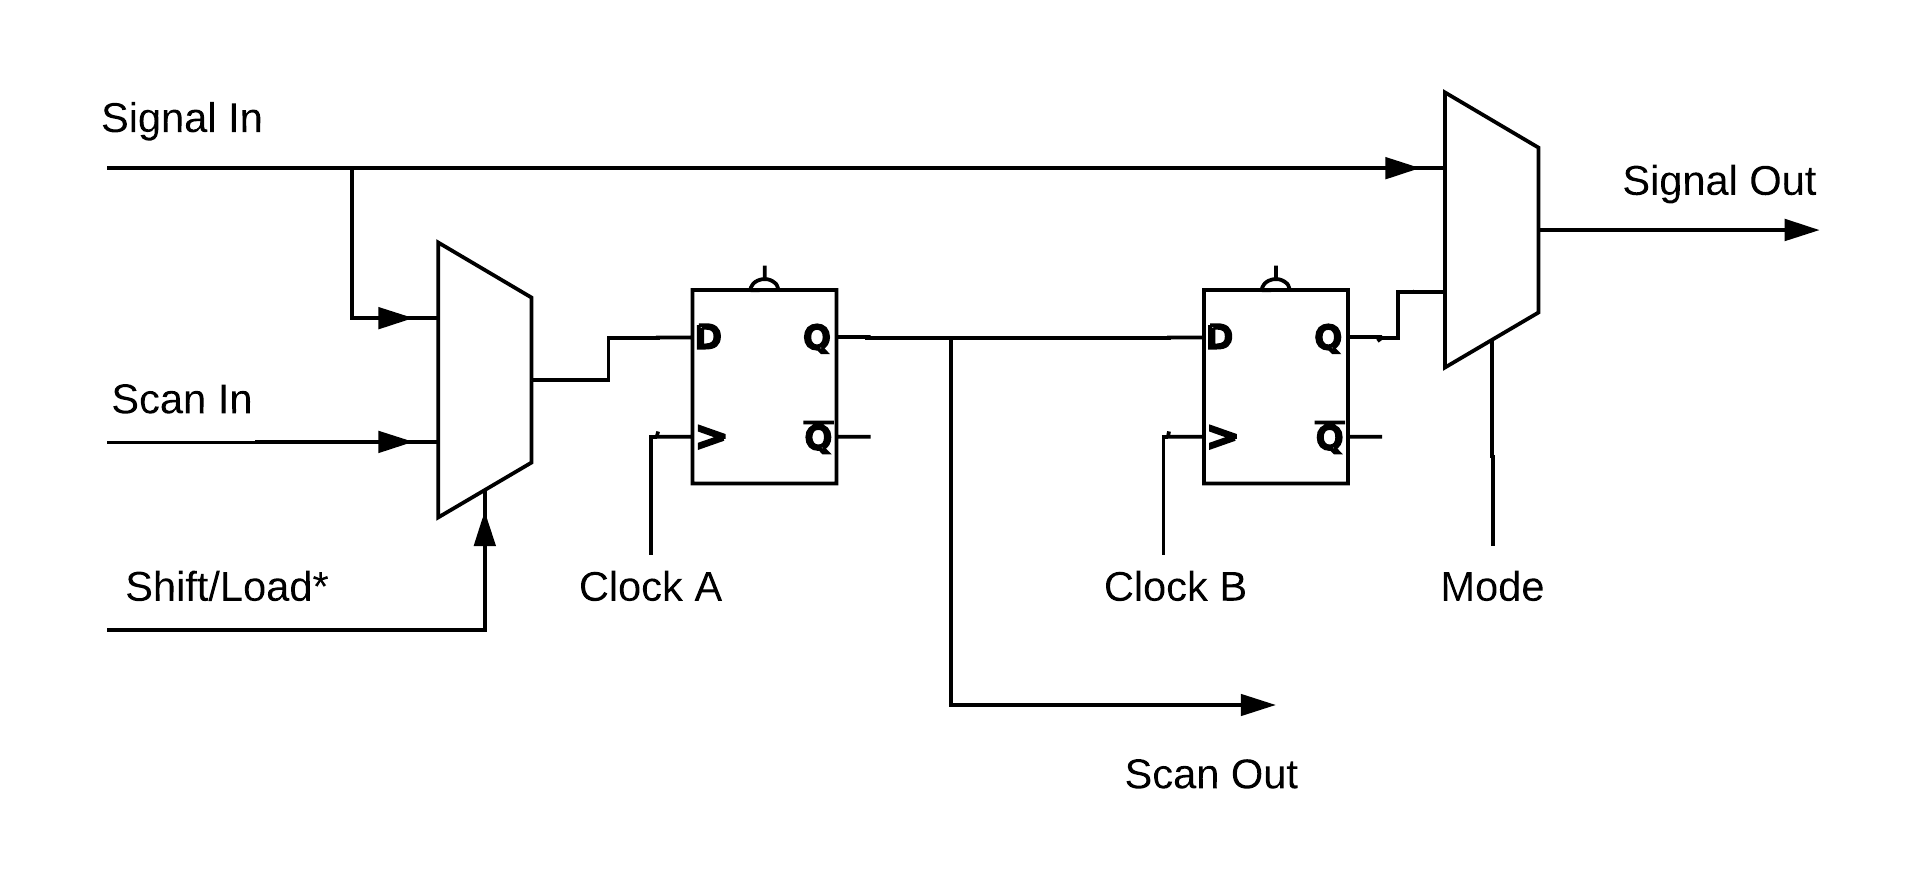
\includegraphics[width=0.8\linewidth]{fig/bscell}
            \caption{Célula de Verificação Periférica}
            \label{fig:bscell}
\end{figure}


O padrão IEEE 1149.1 se baseia em células de teste embutidas em todos os pinos de E/S do circuito integrado (figura \ref{fig:bscell}). As células são encadeadas em uma topologia em anel, um esquema conhecido como \textit{daisy-chain}. O gerenciamento da cadeia de verificação é realizado pela porta de acesso ao teste (ou, em inglês, \textit{test acess port - TAP}), permitindo que todos os pinos de E/S do circuito integrado sejam acessíveis e testados pela porta JTAG. A figura \ref{fig:tap} mostra o esquemático conceitual da lógica interna da porta JTAG. A conexão em \textit{daisy-chain} entre os pinos de um dispositivo com suporte ao IEEE 1149.1 pode facilmente ser estendida para outros integrados compatíveis com o padrão, possibilitando o teste de múltiplos circuitos integrados através de um único conector (figura \ref{fig:cadeiabs}). Como boa prática de DfM, recomenda-se a escolha de integrados que atendam ao padrão.

\begin{figure}
    \centering
        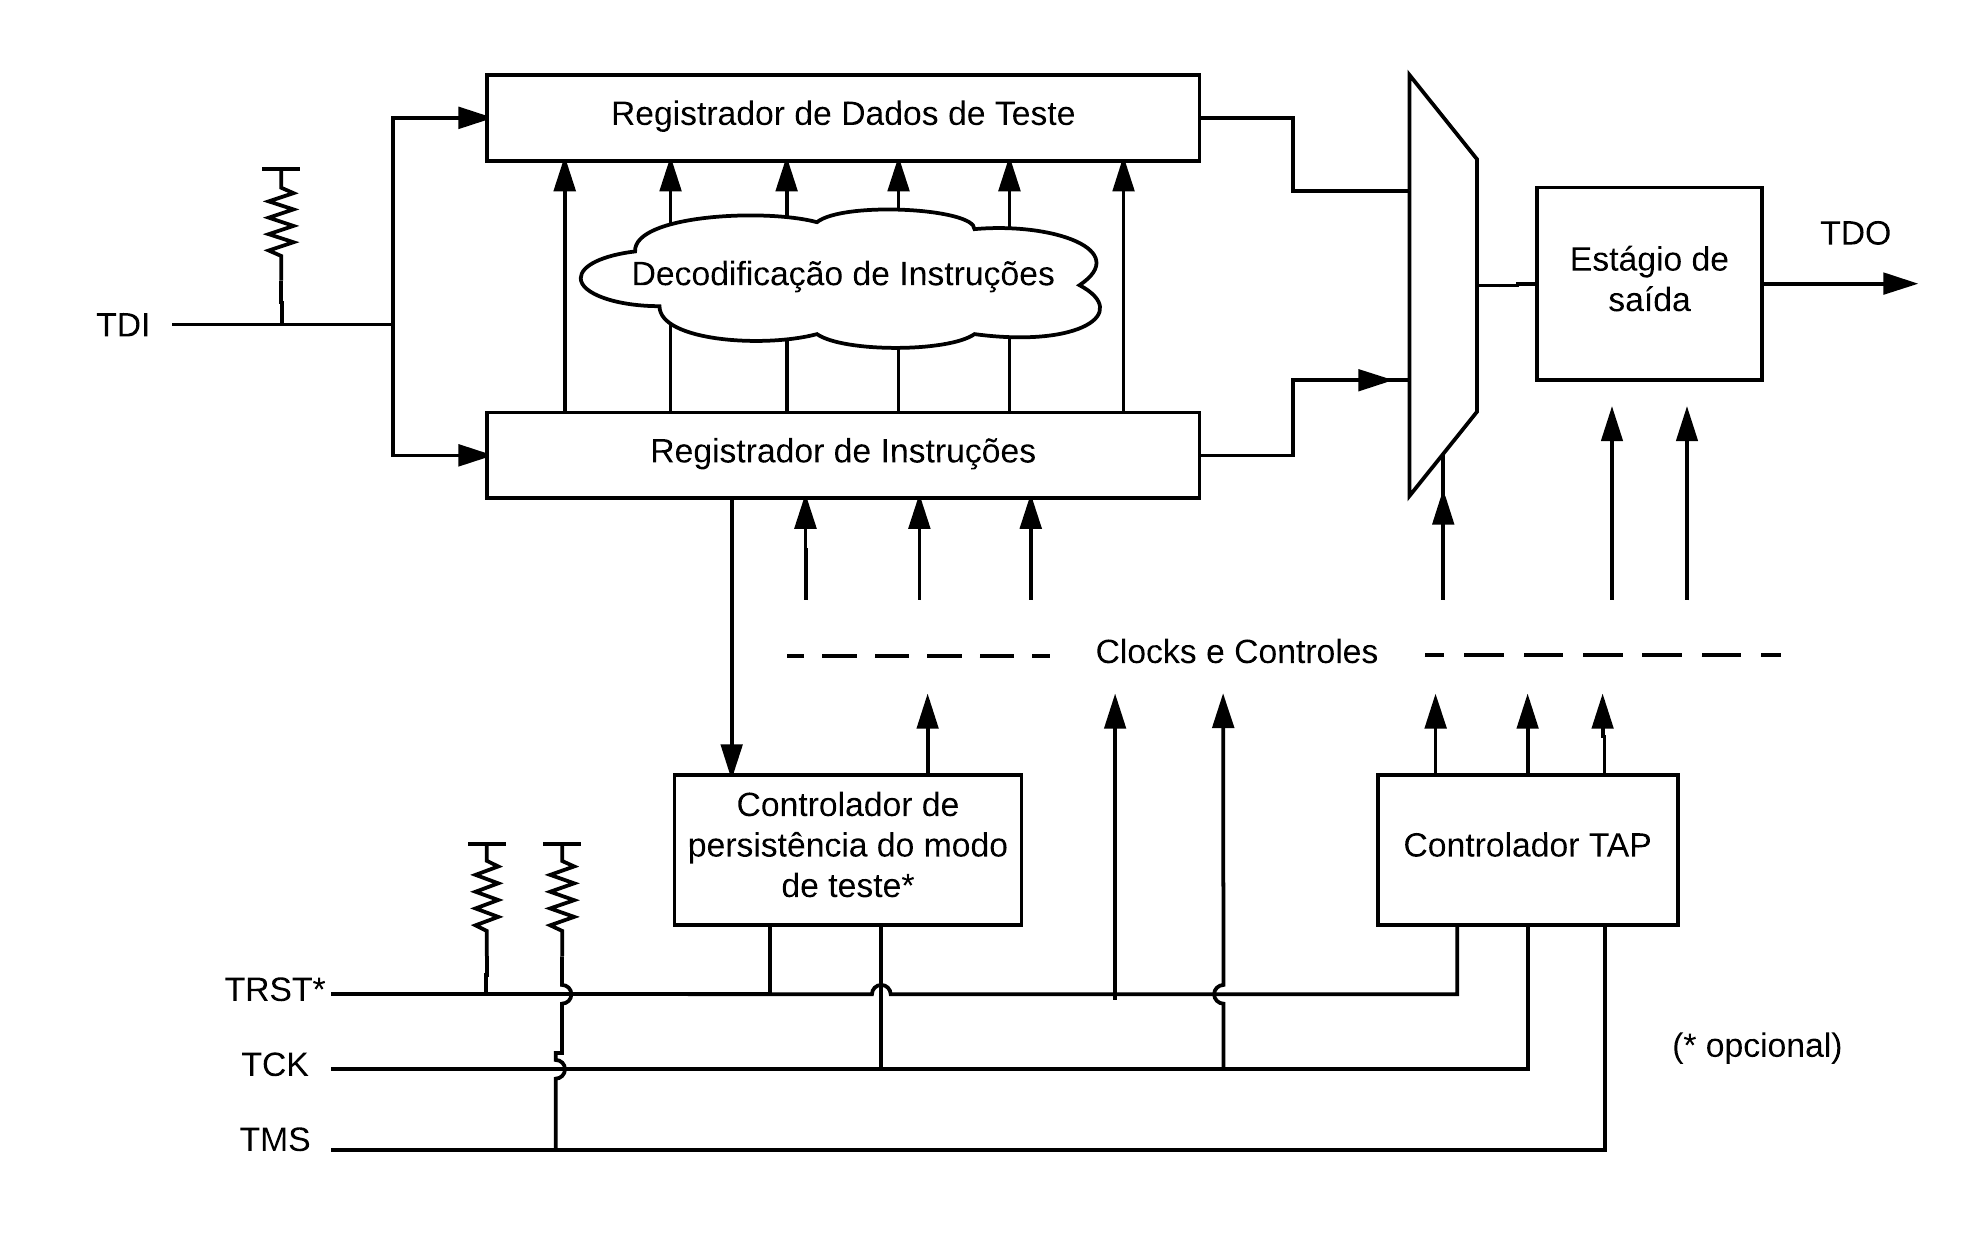
\includegraphics[width=1.0\linewidth]{fig/TAP}
            \caption{Esquemático conceitual da lógica de teste \textit{on-chip}}
            \label{fig:tap}
\end{figure}

Outro componente importante do JTAG é a linguagem de descrição de varredura periférica (BSDL em inglês), que foi inserida numa revisão posterior do IEEE 1149.1 \citep{ieee11491de94}. A BSDL é um subconjunto do VHDL e é voltada para a descrição da infraestrutura de teste de um CI com o objetivo de tornar mais consistente a geração de testes e toda a cadeia de desenvolvimento envolvida nisso.

\begin{figure}
    \centering
        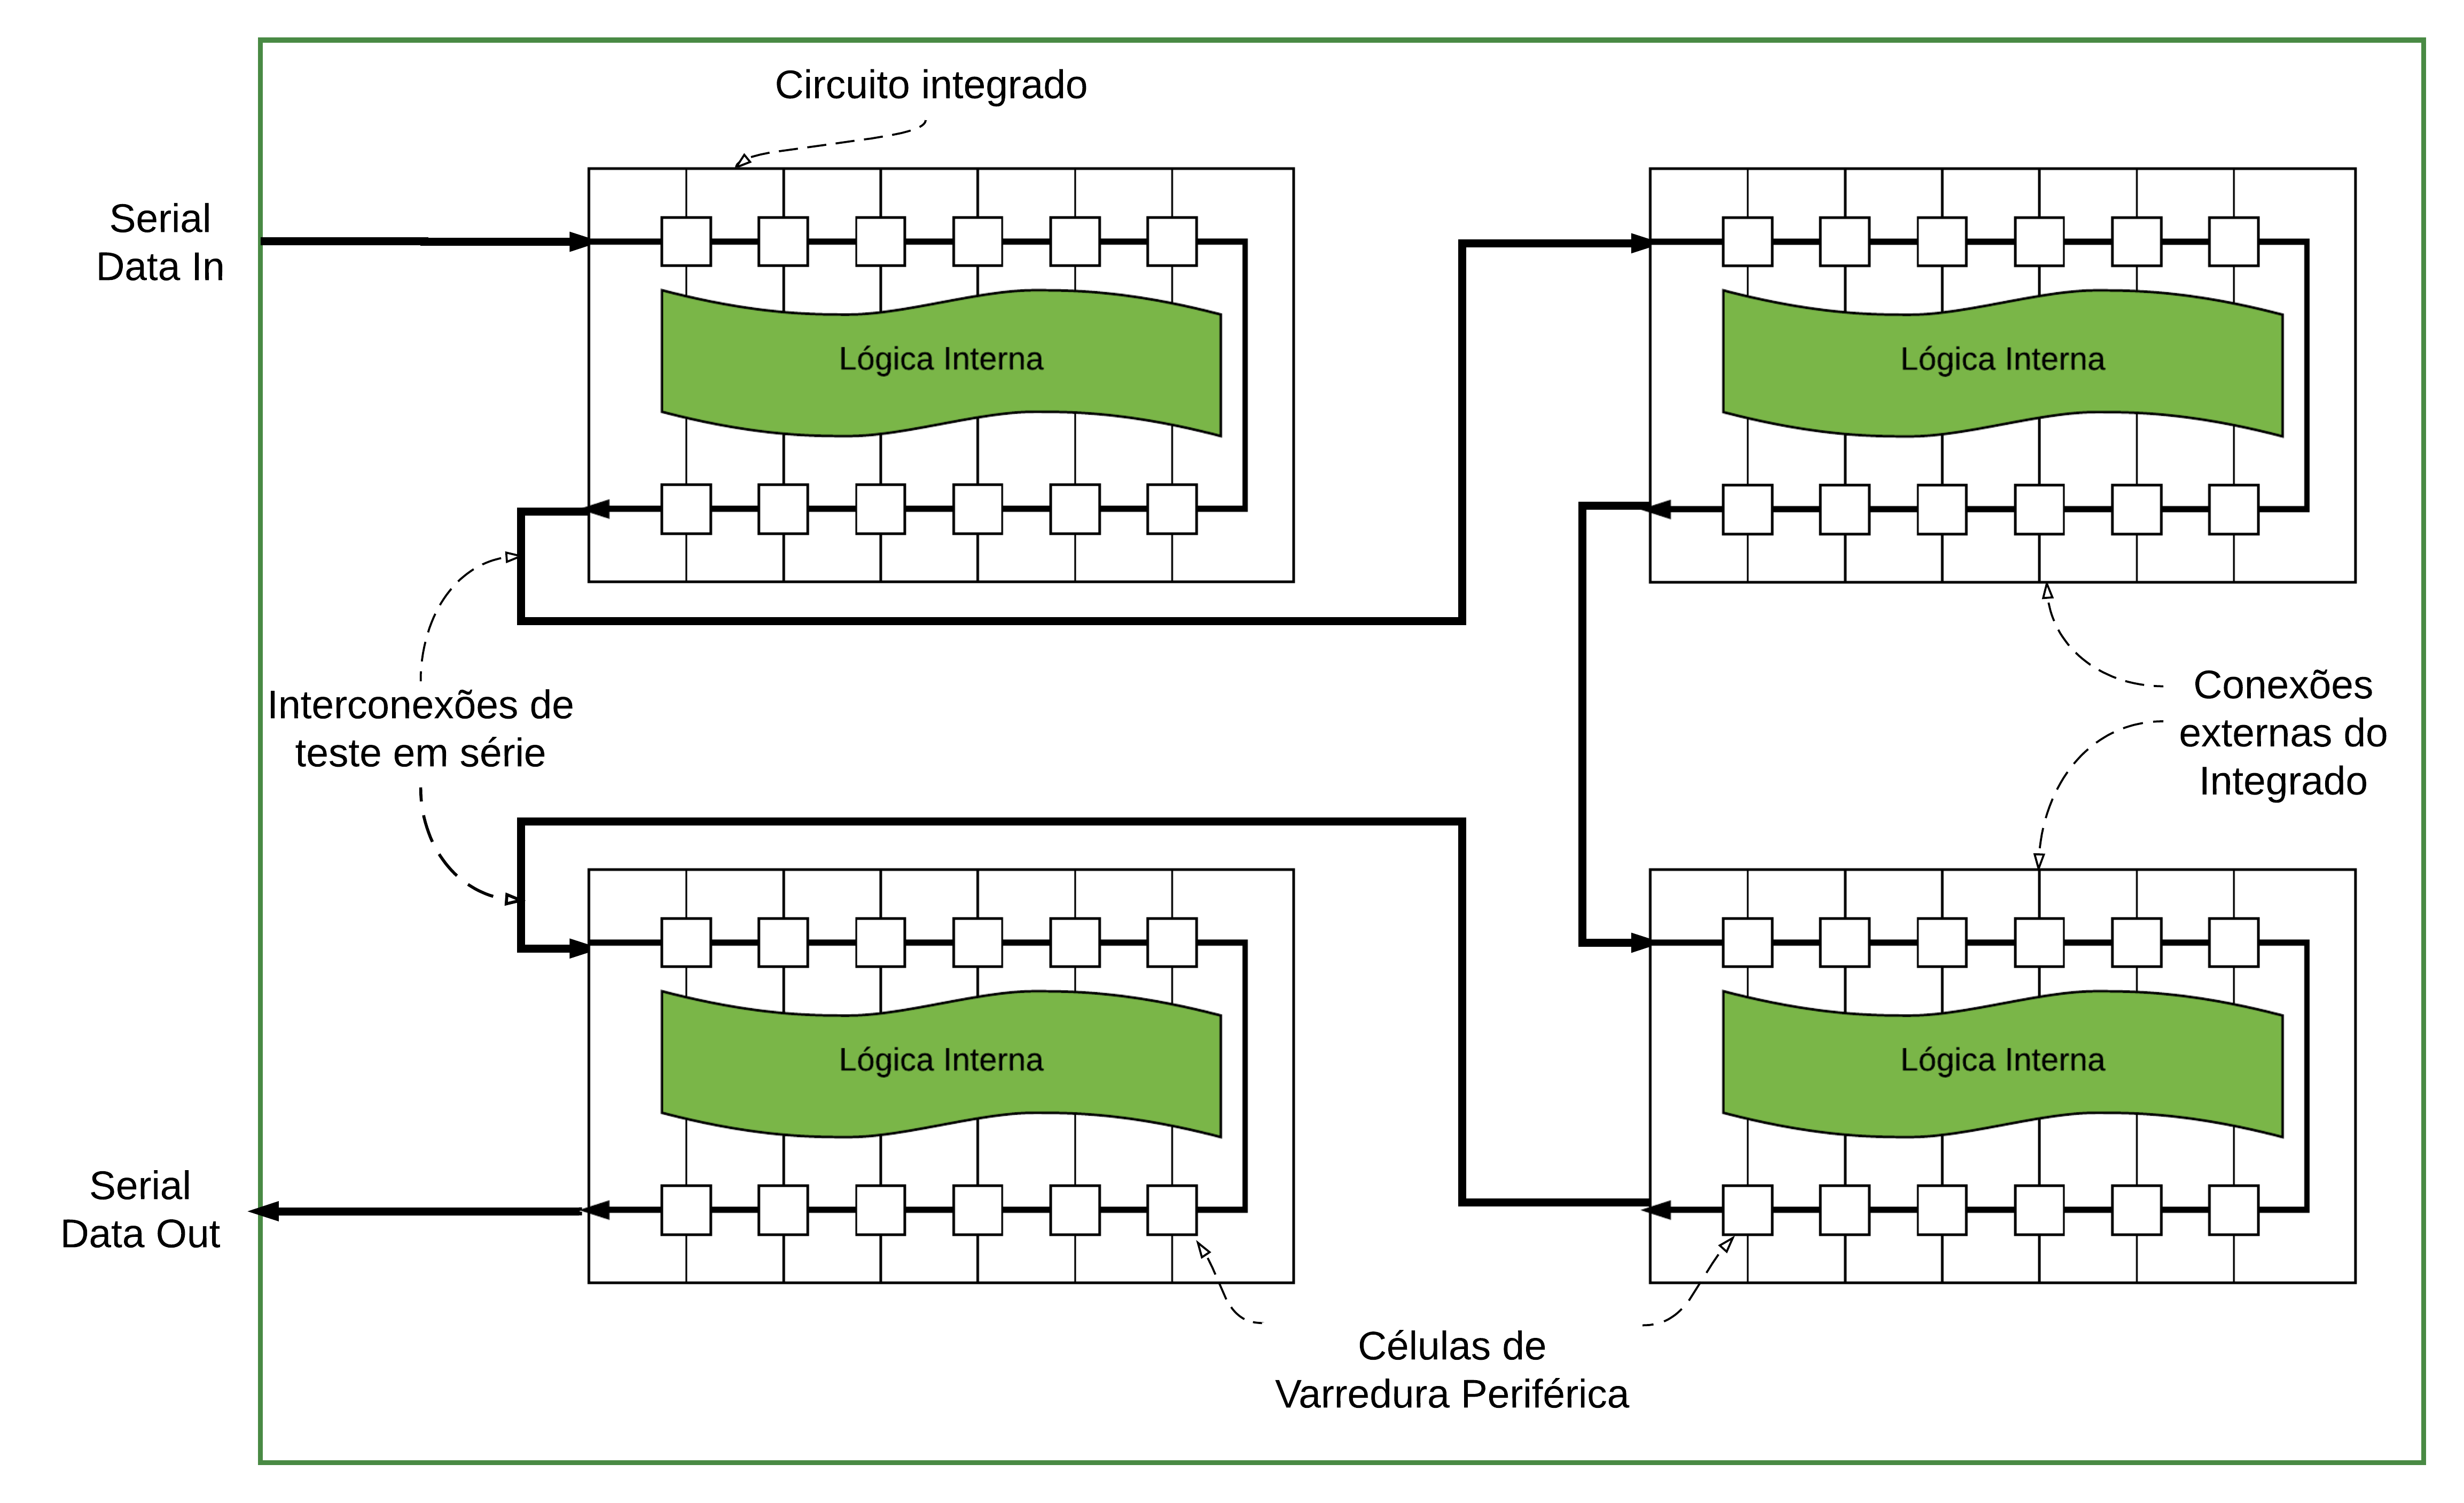
\includegraphics[width=1.0\linewidth]{fig/cadeiabs}
            \caption{PCI com as portas JTAG em \textit{daisy-chain}}
            \label{fig:cadeiabs}
\end{figure}


O padrão IEEE 1149.1 serviu de base para a criação de uma família de padrões de varredura periférica, que são exibidos na tabela \ref{tab:boundaryscanfamily} - adaptada de \citet{jutman2014high}.  

\begin{table}[h]
\centering
\tiny
\caption{Padrões IEEE de varredura periférica \citep{jutman2014high}}
\label{tab:boundaryscanfamily}
\begin{tabular}{p{50}p{50}p{50}p{50}}
\hline
\rowcolor[HTML]{C0C0C0} 
\multicolumn{1}{|p{50pt}|}{\cellcolor[HTML]{C0C0C0}\textbf{Foco principal de aplicação}} & \multicolumn{1}{p{50pt}|}{\cellcolor[HTML]{C0C0C0}\textbf{Propósito Principal}} & \multicolumn{1}{p{50pt}|}{\cellcolor[HTML]{C0C0C0}\textbf{Base da Tecnologia}}    & \multicolumn{1}{p{50pt}|}{\cellcolor[HTML]{C0C0C0}\textbf{Classes de falta a serem cobertas}}     \\
\rowcolor[HTML]{656565} 
\multicolumn{4}{|l|}{\cellcolor[HTML]{656565}{\color[HTML]{FFFFFF} \textbf{IEEE 1149.1 - Boundary Scan \citep{ieee11491old, ieee11491yr2013}}}}                                                                                        \\
\multicolumn{1}{|p{50pt}|}{Teste de Manufatura de PCI}                                        & \multicolumn{1}{p{50pt}|}{Melhorias de acesso aos testes}                               & \multicolumn{1}{p{50pt}|}{Registradores de sondagem on-chip}                            & \multicolumn{1}{p{50pt}|}{Faltas em pinos e integridade de circuto}                                 \\
\rowcolor[HTML]{656565} 
\multicolumn{4}{|l|}{\cellcolor[HTML]{656565}{\color[HTML]{FFFFFF} \textbf{IEEE 1149.4 - Barramento para testes de sinais mistos \citep{ieee11494}}}}\\

\multicolumn{1}{|p{50pt}|}{Medição de sinais analógicos} &
\multicolumn{1}{p{50pt}|}{Melhorias de acesso aos testes} & 
\multicolumn{1}{p{50pt}|}{Chaves \textit{on-chip}} &
\multicolumn{1}{p{50pt}|}{Valores paramétricos}\\

\rowcolor[HTML]{656565} 
\multicolumn{4}{|l|}{\cellcolor[HTML]{656565}{\color[HTML]{FFFFFF} \textbf{IEEE 1149.6 - Teste BST de Redes Digitais Avançadas \citep{ieee11496}}}}\\

\multicolumn{1}{|p{50pt}|}{Teste de redes LVDS de alta velocidade} &
\multicolumn{1}{p{50pt}|}{Teste de malhas acopladas em corrente alternada} & 
\multicolumn{1}{p{50pt}|}{Geradores de pulsos \textit{on-chip}} &
\multicolumn{1}{p{50pt}|}{integridade de malha}\\

%\rowcolor[HTML]{656565} 
\multicolumn{4}{|l|}{\cellcolor[HTML]{656565}{\color[HTML]{FFFFFF} \textbf{IEEE 1149.7 - Pinos reduzidos e TAP aprimorado \citep{ieee11497}}}}\\

\multicolumn{1}{|p{50pt}|}{Teste de placa e depuração de software} &
\multicolumn{1}{p{50pt}|}{Acesso à teste flexivel e em alta velocidade por dois pinos} & 
\multicolumn{1}{p{50pt}|}{SERDES, endereçamento} &
\multicolumn{1}{p{50pt}|}{Contempla todos acima}\\

%\rowcolor[HTML]{656565} 
\multicolumn{4}{|l|}{\cellcolor[HTML]{656565}{\color[HTML]{FFFFFF} \textbf{IEEE 1149.8.1 - Alternância de pinos e sensoriamento sem contato\citep{ieee114981}}}}\\

\multicolumn{1}{|p{50pt}|}{Teste de interconexão de PCIM} &
\multicolumn{1}{p{50pt}|}{Ligações para componentes passivos} & 
\multicolumn{1}{p{50pt}|}{chapas de sensoriamento capacitivo} &
\multicolumn{1}{p{50pt}|}{Circuitos abertos: AC e DC }\\

\multicolumn{4}{|l|}{\cellcolor[HTML]{656565}{\color[HTML]{FFFFFF} \textbf{IEEE P1149.10- TAP de alta velocidade \citep{ieeep1149102016} }}}\\

\multicolumn{1}{|p{50pt}|}{O mesmo que todos acima} &
\multicolumn{1}{p{50pt}|}{Permutação de dados de teste em alta velocidade} & 
\multicolumn{1}{p{50pt}|}{Reuso de pinos I/O de alta velocidade} &
\multicolumn{1}{p{50pt}|}{O mesmo que todos acima}\\

\multicolumn{4}{|l|}{\cellcolor[HTML]{656565}{\color[HTML]{FFFFFF} \textbf{IEEE 1500 - Teste de núcleo embarcado \citep{ieee1500}}}}\\

\multicolumn{1}{|p{50pt}|}{Teste à nível de SoC e IP} &
\multicolumn{1}{p{50pt}|}{Acesso ao teste de \textit{IP cores} em um SoC} & 
\multicolumn{1}{p{50pt}|}{invólucros de núcleos} &
\multicolumn{1}{p{50pt}|}{Faltas no domínio digital dentro de um CI}\\

\multicolumn{4}{|l|}{\cellcolor[HTML]{656565}{\color[HTML]{FFFFFF} \textbf{IEEE 1687 - Acesso por Instrumentação Embarcada \citep{ieee1687}}}}\\

\multicolumn{1}{|p{50pt}|}{Teste de CI, depuração, diagnóstico} &
\multicolumn{1}{p{50pt}|}{Padrão de acesso por instrumento} & 
\multicolumn{1}{p{50pt}|}{Cadeias de sonda reconfiguráveis} &
\multicolumn{1}{p{50pt}|}{Específicas do instrumento}\\

\multicolumn{4}{|l|}{\cellcolor[HTML]{656565}{\color[HTML]{FFFFFF} \textbf{IEEE P1838 - Acesso a teste para CIs 3D \citep{ieeep18382016}}}}\\

\multicolumn{1}{|p{50pt}|}{Teste de integração 3DSIC} &
\multicolumn{1}{p{50pt}|}{Acesso à teste através das vias TSV} & 
\multicolumn{1}{p{50pt}|}{O mesmo que os padrões 1500, 1149.1, 1687} &
\multicolumn{1}{p{50pt}|}{Integridade das vias TSV}\\
\hline


\end{tabular}
\end{table}

O padrão IEEE 1149.4 \citep{ieee11494} foi criado para testes paramétricos de componentes passivos, resistores pull-ups, componentes ativos como diodos, transistores e de redes de impedância. Serve como uma extensão da varredura periférica para sinais analógicos. Este padrão ainda tem um número limitado de dispositivos compatíveis.

Já o padrão IEEE1149.6 \citep{ieee11496} estende a varredura periférica a portas de comunicação com acoplamento em corrente alternada, como por exemplo, portas que atendem ao padrão de LVDS, operando em paralelo com os padrões 1149.1 e 1149.4. O que possibilita esta tecnologia são as inserções de geradores de pulso nos pinos de saída e \textit{receivers} CA comuns e diferenciais nas entradas dos dispositivos que dão suporte a este padrão.

É possível citar outros exemplos significativos, como é o caso do IEEE1149.7 - cJTAG \citep{ieee11497}. Este padrão opera em pinos reduzidos e possibilita uma topologia em estrela ao invés do \textit{daisy-chain}, permitindo um acesso mais rápido, além de oferecer uma infraestrutura adicional de suporte a tecnologias mais avançadas. O IEEE P1687 \citep{ieee1687} introduz o conceito de instrumentação embarcada para a aplicação de tarefas de teste, medição e diagnóstico, assunto abordado na próxima seção.

\subsection{Teste Controlado por FPGA ou Processador e Instrumentação Embarcada}
\label{FCT}

Conforme mencionado anteriormente, o JTAG não permite o uso de padrões de teste em velocidade nominal, deixando a classe de falhas de desempenho sob responsabilidade de testes funcionais. Atualmente, parte da indústria tem utilizado os componentes centrais de seus sistemas, como por exemplo os FPGAs e microcontroladores, como dispositivos de teste embarcado \citep{alcrouch2011, thomaswenzel2013}, cunhando os termos \textit{FPGA-Controlled Test - FCT} e \textit{Processor-Controlled Test - PCT}. 

 Além de cobrir os testes em domínio CA, como atrasos e \textit{crosstalk}, ainda possibilitam um acesso de baixo nível no sistema, já que esses são normalmente componentes centrais do projeto. O custo marginal é ínfimo, já que o todo o hardware de teste é reutilizado do produto e a memória de teste é apagada, voltando o dispositivo para sua funcionalidade original. \citet{jutman2014high} afirmou que ainda são poucas as empresas que fornecem ferramentas automatizadas para esta classe de testes.

O conceito de teste controlado por FPGA é possibilitado pelo uso de instrumentos embarcados, que são definidos como qualquer estrutura lógica dentro de um dispositivo cuja função é de teste, diagnóstico, \textit{Design for Testability (DfT), Design for Debug  (DfD), Design for Yield (DfY),} e outros. Neste escopo, enquadram-se diversas estruturas lógicas:    
\begin{itemize}
    \item Testadores de memória e BIST/BISD;
    \item Analisadores de taxa de erro (BERT) em canais de comunicação;
    \item Geradores de padrões de teste e \textit{buffers} de captura digital;
    \item Caracterizadores e Calibradores de E/S complexas;
    \item Testadores de barramentos de comunicação LAN, SATA, PCI, CAN, LIN, I2C, SPI e UART;
    \item Testadores sistêmicos e programação de memórias não voláteis;
    \item Instrumentos definidos por usuário.
\end{itemize}

\citet{Stollon2011} mostra que estas estruturas de instrumentação embutida surgiram, em parte, pela necessidade de medições que causem menos interferências ou que não comprometam a integridade do sinal de barramentos de alta velocidade, internos ou externos ao CI. Dessa forma, os fabricantes passaram a embutir núcleos de propriedade intelectual - \textit{IP cores} - de instrumentação interna, permitindo testes não intrusivos e facilitando a validação e diagnóstico de placas.

Originalmente, cada um destes instrumentos são acessados e gerenciados por uma variedade de instrumentos externos, usando diversos mecanismos e protocolos. Isso dificulta a integração entre CIs e o reuso de tecnologia e equipamento. Logo, existia uma necessidade de padronização destes protocolos, de forma a garantir uma metodologia eficiente e organizada para a preparação de testes e para o acesso e controle destes instrumentos embarcados. 

O IEEE 1687 \citep{ieee1687}, também conhecido como \textit{Internal JTAG } ou IJAG, foi o padrão criado para definir e descrever as interfaces de acesso à instrumentação embarcada pela porta padrão IEEE1149.1, possibilitando a realização de testes avançados e não intrusivos em uma PCI inteira pela porta JTAG. Como ilustrado na figura \ref{fig:ieee1687}, o IJTAG não define os instrumentos ou suas funcionalidades por si, mas sim os padrões de infraestrutura de acesso e como descrever os métodos e funcionalidades dos instrumentos. Isso se consolidou em duas linguagens de descrição dentro deste padrão: uma para as características destas funcionalidades, a PDL \textit{(procedural description language)}, e outra para os requerimentos de interface com estas funcionalidades - ICL \textit{(instrument connectivity language)}. Estas duas linguagens de descrição - PDL e ICL - facilitam o reuso e a descoberta de qualquer instrumento que seja compatível com o padrão IEEE 1687, independente do seu tipo, propósito ou origem. 

\begin{figure}
    \centering
        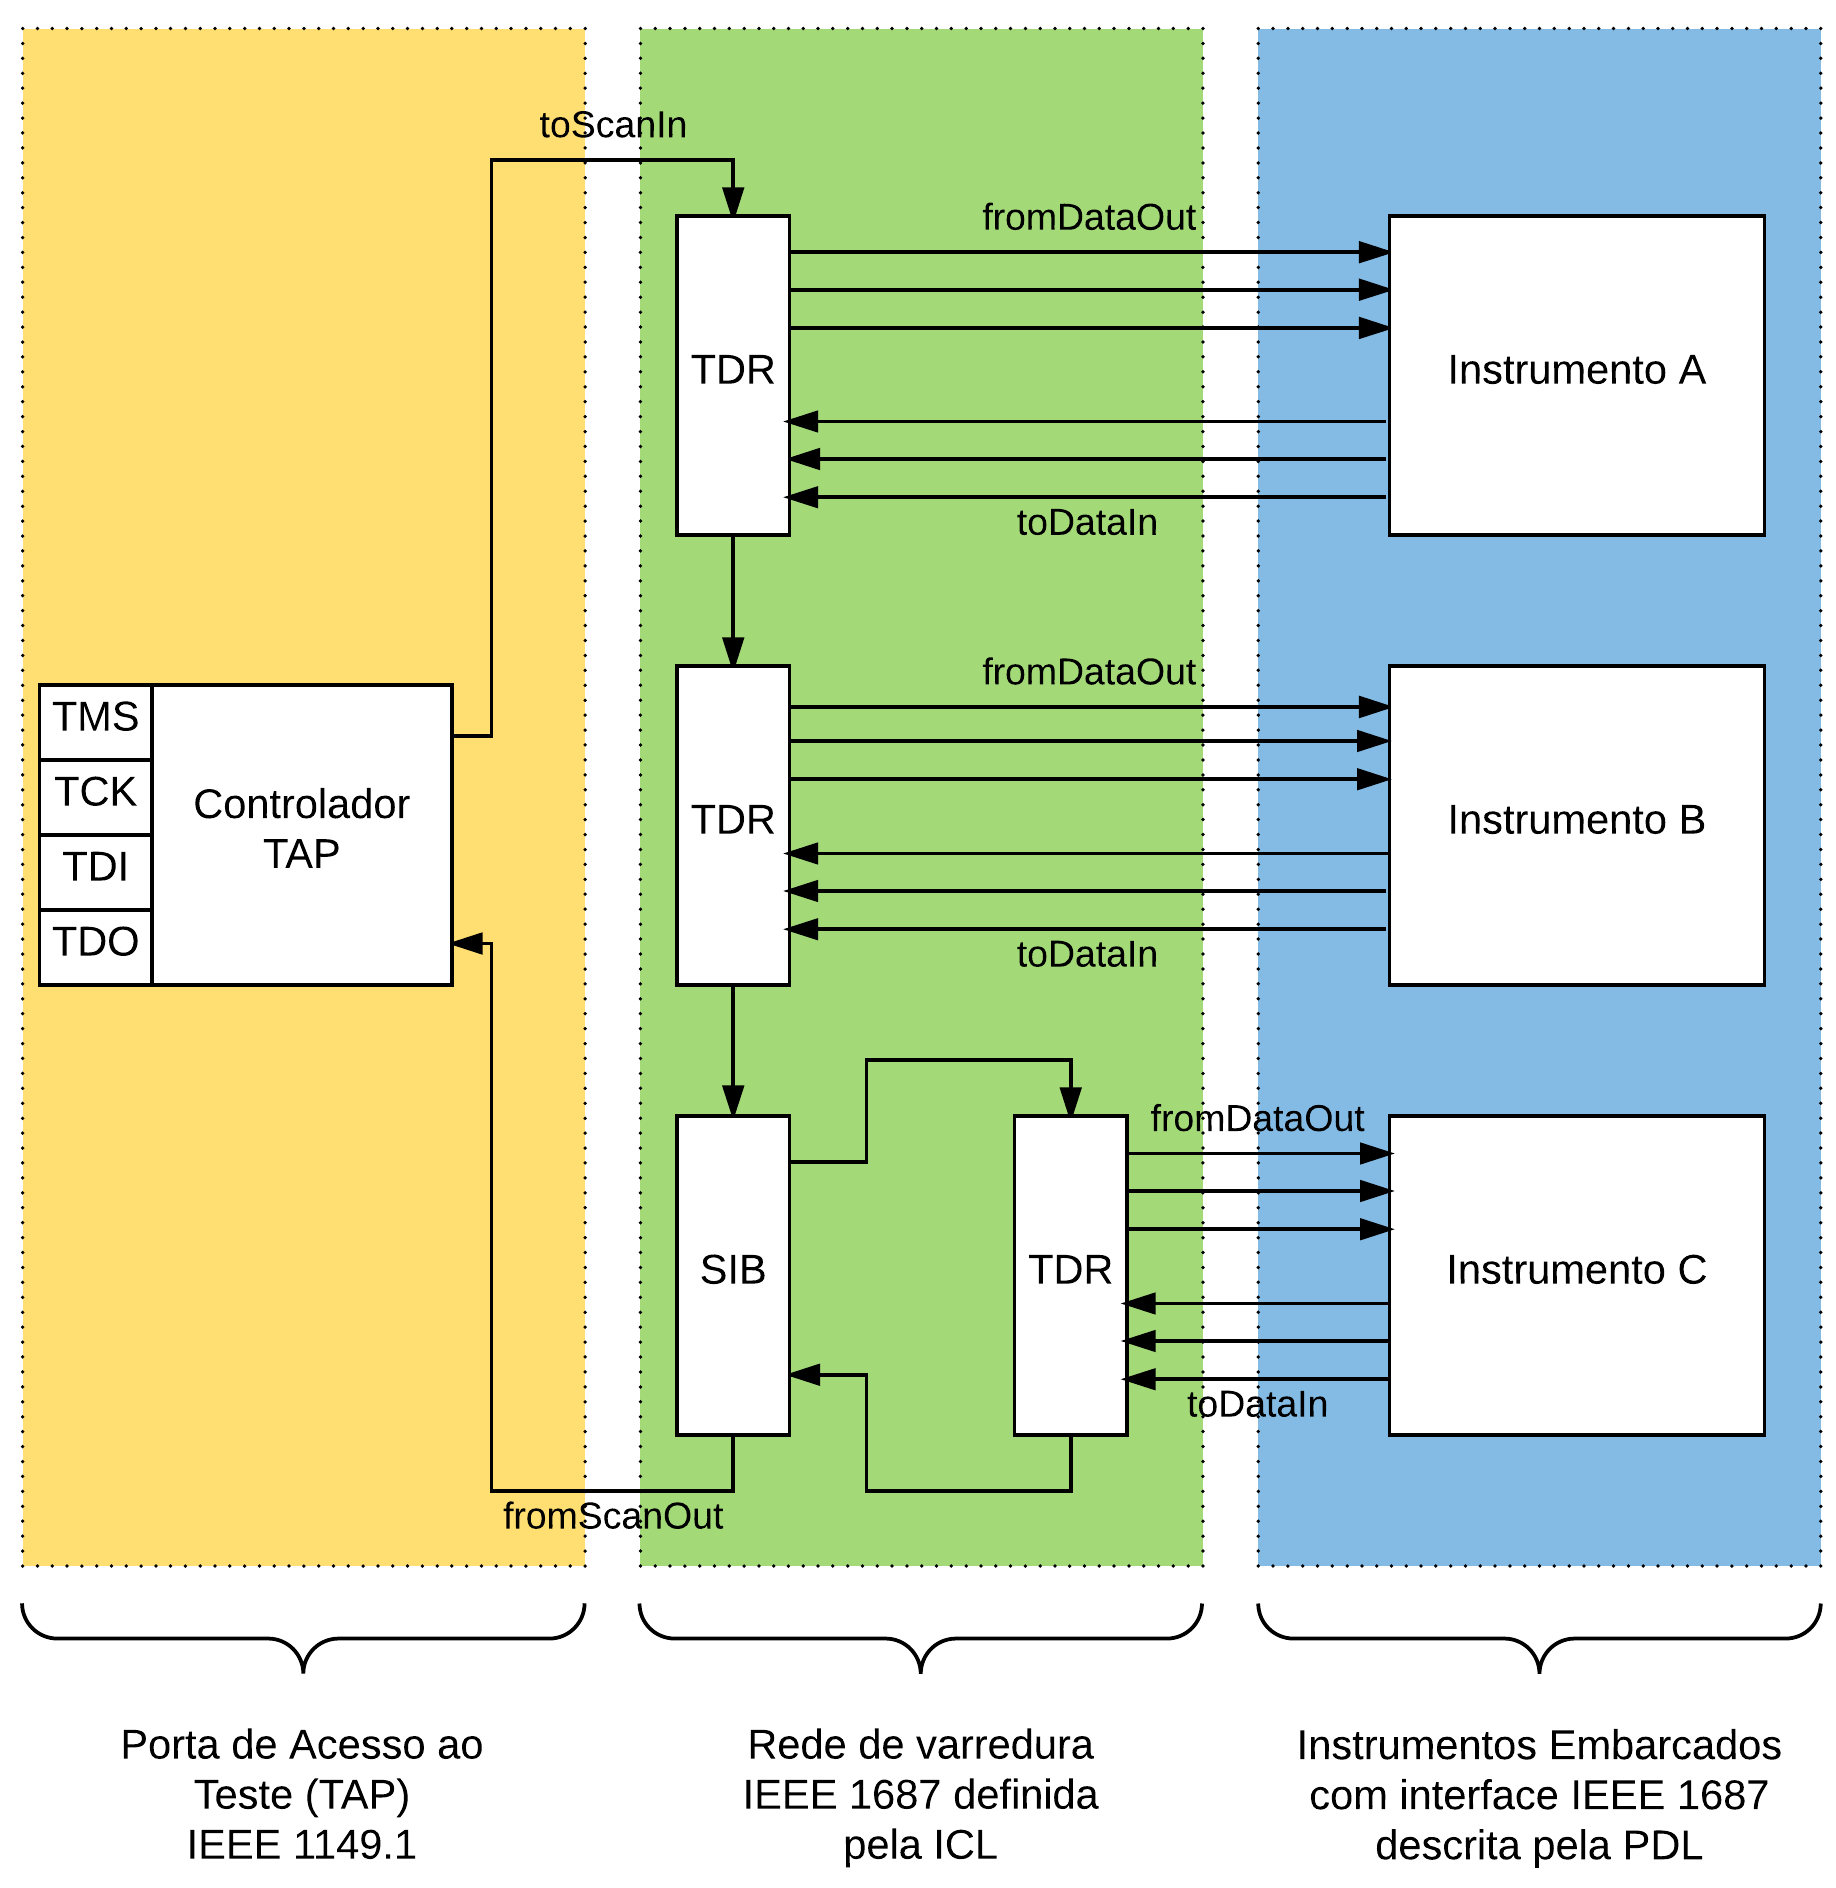
\includegraphics[width=1.0\linewidth]{fig/IEEE1687}
            \caption{Rede IEEE 1687 conceitual de múltiplas cadeias de varredura}
            \label{fig:ieee1687}
\end{figure}

Dessa forma, o padrão IEEE 1687 funciona como uma extensão do IEEE 1149.1, de maneira que a porta JTAG de um CI ou uma placa possa ser usada para configurar, operar, e coletar dados de instrumentos embarcados.

Os FCT e PCT aliados ao IEEE 1687 oferecem uma cobertura em múltiplos domínios de falta (estruturais, CC, CA e faltas de desempenho), reduzindo ou até mesmo superando a necessidade de equipamentos de teste especializados \citep{thomaswenzel2013}. Em \citet{jutman2014high} observa-se que isso possibilita não só uma manufatura e teste de produção mais baratos e descomplicados, como também abre porta para o reuso dos testes em campo para o diagnóstico de falhas operacionais, o que não só reduz os custos logísticos de transporte de equipamentos especializados para depuração e diagnóstico, como possibilita que testes avançados sejam realizados sob condições reais de operação. 

\subsection{Teste Funcional}
% https://pad.riseup.net/p/RwPsE9imTtNzadskjasdoqidjefkadf
%definição
Define-se teste funcional como aquele que não depende da estrutura interna de DfT de um sistema, mas sim das portas de entrada e saída \citep{jutman2014high}. Outra definição, formulada pelo mesmo autor, é a de um teste que se baseia somente nas informações funcionais do sistema, sem conhecimento da estrutura interna. Essas duas definições se interseccionam na maioria das vezes.

% APLICAÇÕES
% quero dizer que em todos autores é unanime que
O teste funcional serve para complementar objetivos específicos de teste, sendo normalmente empregado como etapa final de linha de produção \citep{thibeault2006,jutman2014high,tumim2001}. A tendência é que o teste funcional, devido aos seus custos crescentes, perca espaço com a adesão e popularização dos padrões mais avançados de varredura periférica e instrumentação embarcada, limitando-se a atingir certos objetivos específicos de teste que não podem ser cobertos por testes de varredura \citep{thibeault2006, thomaswenzelenricozimmermann2016}. 

Entretanto, existem casos onde o suporte ao IEEE 1149.1 é inexistente e o teste funcional é a única opção para validação do produto. \citet{tumim2001} afirma que, mesmo com os últimos avanços nos testes de varredura periférica, o teste funcional ainda é insubstituível. Vale lembrar da relação complementar entre essas duas categorias de teste, ilustrada pela figura \ref{fig:cobertura}. 

\citet{jutman2014high} elenca outras aplicações de testes funcionais, dentre elas: a inspeção de recebimento de componentes de terceiros (por exemplo: uma fonte de alimentação feita por outro fabricante, ou circuito integrado de alto valor) e em casos de teste em campo do circuito eletrônico, quando se depende de equipamento externo especializado para a realização de testes ou o fabricante original do CI não disponibiliza o acesso à infraestrutura de teste interna.

%vantagens e desvantagens reescrever
%\citet{thibeault2006} enumera algumas das principais vantagens e desvantagens do teste funcional, destacando-se: 

Destacam-se dentre as principais vantagens do teste funcional:
\begin{itemize}
    \item A possibilidade de execução de testes em velocidade nominal de operação, possibilitando a detecção de defeitos relacionados a temporização \citep{thibeault2006};  
    \item Verificações funcionais que garantam que o projeto opera como prometido,  coisa que testes estruturais e de varredura não conseguem fazer \citep{tumim2001}.
\end{itemize}

Já entre as desvantagens: 

\begin{itemize}
    \item O processo de teste funcional em velocidade nominal é muito mais demorado, se comparado com a varredura periférica \citep{thibeault2006}; 
    \item O esforço e o tempo requerido para gerá-los podem ser significativos e a dificuldade cresce exponencialmente em relação ao número de portas lógicas. Essa dificuldade persiste ainda que existam algoritmos para o teste funcional das estruturas lógicas mais comuns, como CPUs, MMUs, BPU, processadores multicores e GPUs.
\end{itemize}
 
%o que compõe
Como um sistema caixa preta, o teste funcional é composto por dados de excitação, a saída resultante do teste e também um roteiro de teste. Em abordagens tradicionais, o teste funcional de interfaces com periféricos e interconexões é gerenciado por um ATE para estímulos e observação. Este esquema está representado no diagrama da figura \ref{fig:funcblock}. Em casos de manutenção em campo ou local de difícil acesso, pode-se utilizar uma conexão de \textit{loopback} no dispositivo.

\begin{figure}[h!]
    \centering
        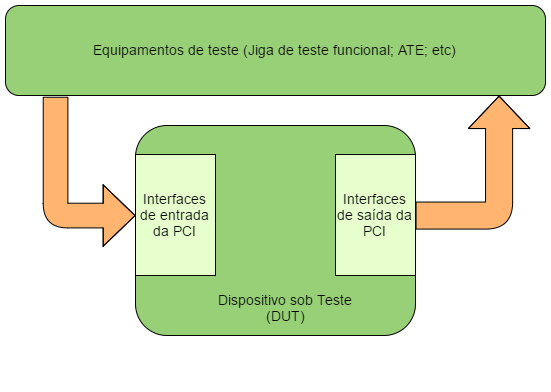
\includegraphics[width=0.8\linewidth]{fig/functionaltest}
            \caption{Diagrama de blocos de um esquema de teste funcional}
            \label{fig:funcblock}
\end{figure}

%geração de roteiros e estado da arte
A geração do roteiro de teste geralmente é manual e os esforços de pesquisa em teste funcional se concentram em métodos de automatização da geração de testes. O trabalho de \citet{thibeault2006} propõe uma investigação em otimização de roteiros e reuso de padrões de teste gerados diretamente por ferramentas de validação de projeto. 

Também existem trabalhos mais recentes de automatização de testes funcionais, como o de \citet{riefert2014effective}, que desenvolveu um método automatizado para testes funcionais em processadores utilizando métodos formais.


%Em \citep{thibeault2006} ve-se que que é importante considerar que, mesmo com suas vantagens, é crescentemente difícil justificar o uso de testes funcionais em velocidade nominal como abordagem principal. Sob esta perspectiva, parece que um teste funcional em velocidade nominal será mais e mais restrito à partes do DuT sem suporte à varredura periférica \citep{thibeault2006}. Todavia, a captura de defeitos relacionados à temporização não é o único aspecto positivo do teste funcional. Sua natureza não serial também pode ser explorada para propósitos de otimização de testes. Em [But100], foi proposto a criação de um pequeno conjunto de padrões de teste moderadamente rápidos, inseridos de inicio no programa de teste, de maneira a obter vantagem de sua inicial má capacidade de detecção de dispositivos enquanto mantem custos de desenvolvimento a um nível aceitável. Estas propostas foram baseadas no fato de qeu é mais difícil e caro criar e depurar padrões quando a frequência do  padrão funcional é perto da velocidade especificada do dispositivo.

\section{Padrões de projeto em LabVIEW}

Padrões de projeto são formas bem estabelecidas para resolver problemas comumente recorrentes. Não se trata de um código fonte ou \textit{framework}, mas de uma descrição de como se resolver um problema que pode ser aplicado em diversas situações. Padrões de projeto ganharam popularidade na ciência da computação após a obra de \citet{gamma1994design}. 

As vantagens de usá-los estão na facilidade dos desenvolvedores em reconhecê-los no código fonte, de dispensarem a necessidade de reinventar soluções para problemas recorrentes, como também na confiança de estar aplicando uma solução bem trabalhada para um tipo de problema.

No caso específico do LabVIEW, os padrões de projeto podem ser um modelo como um \textit{framework}, ou seja, uma base de códigos para o desenvolvimento da aplicação. Em \citet{blume2007labview} descrevem-se os principais padrões de projeto e \textit{frameworks} da linguagem: as máquinas de estado; os laços acionados por evento; o produtor-consumidor; o tratador de mensagem em fila; a máquina de estados em fila; e o Modelo de Atores.

\subsubsection{Máquinas de Estados Finitos}
As máquinas de estados finitos (figura \ref{fig:statemachine}) são amplamente conhecidas e, nelas, o comportamento dinâmico do programa depende de estados cujas transições dependem de uma lógica de estados. É fundamental a criação de uma tabela de estados para uma máquina de estados efetiva.

\begin{figure}
    \centering
        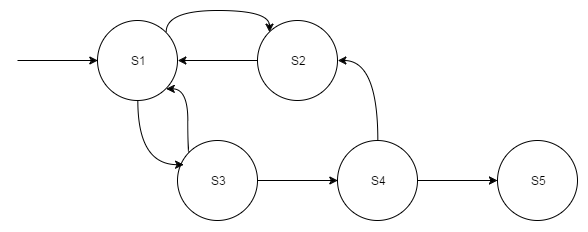
\includegraphics[width=0.8\linewidth]{fig/patt/statemachine}
            \caption{Um exemplo de máquina de estados finita}
            \label{fig:statemachine}
\end{figure}

\subsubsection{Laços Acionados por Eventos}
Nos laços acionados por eventos (figura \ref{fig:eventloop}), diferentemente do paradigma procedural, a execução do programa é decidida em tempo de execução: o programa permanece em estado de espera até a ocorrência de um evento e seu despacho para um tratador. Esta técnica poupa tempo de CPU e é uma boa alternativa ao uso de \textit{pooling}, além de poder ser aplicada em qualquer sistema de acionamento de processos escravos.

\begin{figure}[h]
    \centering
        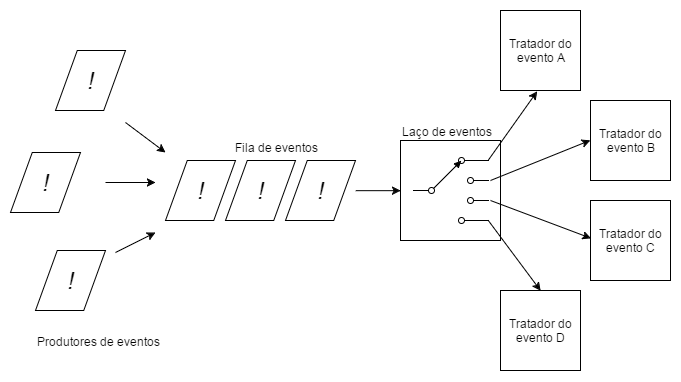
\includegraphics[width=1\linewidth]{fig/patt/eventloop}
            \caption{Laço acionado por eventos}
            \label{fig:eventloop}
\end{figure}

\subsubsection{O Produtor - Consumidor}
O produtor-consumidor (figura \ref{fig:prodcon}) é normalmente aplicado quando se precisa executar tarefas assíncronas e comunicar entre elas sem perda de desempenho, caso uma dependa da outra. Este padrão tem por característica a relação de mestre/escravo entre os laços e a independência no fluxo de dados entre eles. Uma tarefa produzindo dados ou comandos e uma ou mais tarefas consumindo o que a produtora gera. A comunicação entre as tarefas é realizada por filas, ou seja, os dados são enfileirados e desenfileirados em um \textit{buffer}, em esquema conhecido como \textit{first-in-first-out - FIFO}.

\begin{figure}
    \centering
        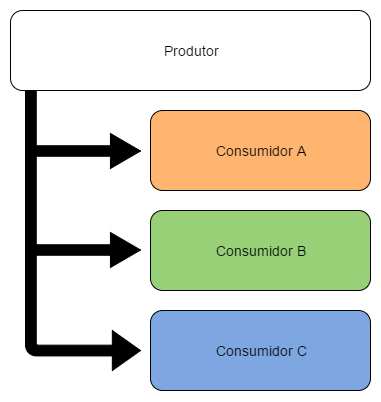
\includegraphics[width=0.5\linewidth]{fig/patt/produtorconsumidor}
            \caption{Diagrama do produtor-consumidor com 4 laços independentes comunicando por uma fila}
            \label{fig:prodcon}
\end{figure}

\begin{figure}
    \centering
        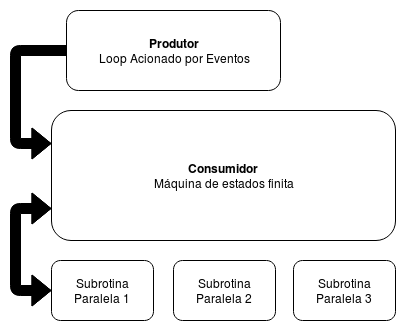
\includegraphics[width=0.7\linewidth]{fig/patt/tmf}
            \caption{Diagrama do tratador de mensagens em fila}
            \label{fig:tmf}
\end{figure}


\subsubsection{Tratador de mensagens em fila}
O tratador de mensagens em fila - TMF (figura \ref{fig:tmf}) ou, em inglês, \textit{Queue Message Handler} ou \textit{Queue-driven State Machine}, é uma extensão do produtor-consumidor, possibilitando que processos escravos possam atuar também como produtores e comunicar entre si. Normalmente apresenta-se como na figura \ref{fig:tmf}, com um laço mestre acionado por eventos criando tarefas, um processo principal e subprocessos auxiliares. O TMF não só é um padrão de projeto, mas também a arquitetura base de muitas aplicações de média a grande complexidade. É usado em aplicações que exijam interfaces de usuário responsivas, aplicações multitarefa e o desacoplamento de processos.


\subsection{Framework de Atores}
\label{actorframework}


%\subsubsection{A necessidade de um outro modelo de computação concorrente}

Na programação imperativa, assim como na maior parte dos paradigmas e linguagens de programação, as \textit{threads} são a solução tradicional para problemas de concorrência. Entretanto, programação concorrente baseada em \textit{threads}, \textit{locks} e estados compartilhados são ditas difíceis de fazer e propensas a erro \citep{Erb2012}. 

Em 1973, \citet{hewitt1973session} criou o modelo de atores como alternativa às \textit{threads} em problemas de computação concorrente e sistemas distribuídos. Sua premissa é a de que qualquer computação fisicamente possível pode ser diretamente implementada usando Atores \citep{hewitt2010actor}. 

 A abordagem no modelo de atores é totalmente diferente, já que retira inteiramente a noção de estado compartilhado. Ainda é possível que haja estados, entretanto, estes estão exclusivamente acoplados a uma única entidade, chamada Ator.

O modelo tem sido usado tanto como uma estrutura base para compreensão de problemas de concorrência, como também como base teórica para diversas implementações práticas de sistemas concorrentes. O crescimento de sistemas concorrentes massivos de computação em nuvem e processadores \textit{multi-cores} tem aumentado o interesse por este modelo. Exemplos de sistemas modelados pelo sistema de atores incluem: sistemas de email, Serviços Web e Objetos com \textit{locks}.

\subsubsection{Conceitos fundamentais do modelo}

Um ator é a unidade primitiva de computação. Ao receber uma mensagem, um ator pode concorrentemente \citep{hewitt2013computation}:

\begin{itemize}
    \item Criar um finito número finito de novos atores;
    \item Enviar finitas mensagens para outros atores;
    \item Designar como tratar a próxima mensagem que receber, alterando seu estado interno.
\end{itemize}

%Comunicação Assíncrona.
Para comunicação, o modelo de atores usa a troca de mensagens assíncronas, atribuindo a cada ator a sua caixa de mensagens (figura \ref{fig:actor}), local onde as mensagens são armazenadas enquanto o ator processa a mensagem anterior. Num sistema de atores, tudo o que um ator sabe do outro é o endereço de sua caixa de mensagens.

O ator sempre trabalha em resposta às mensagens que recebe, tratando-as sequencialmente, uma de cada vez \citep{Erb2012}. Isso significa que, para executar múltiplas mensagens de forma concorrente, será necessário que antes se crie um ator para cada uma delas. 

    \begin{figure}
        \centering
        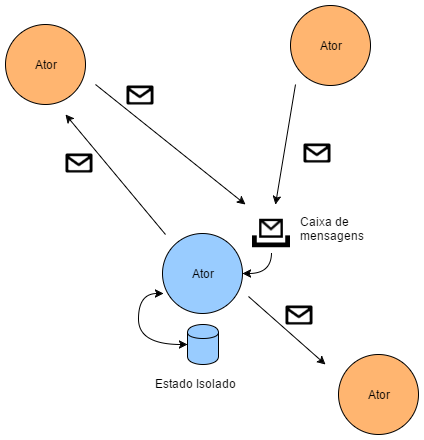
\includegraphics[width=0.9\linewidth]{fig/actor}
        \caption{Um exemplo de uma rede com alguns atores, com destaque para um ator, sua caixa de mensagens e seu estado interno. Adaptado de \citet{Erb2012}}
        \label{fig:actor}
    \end{figure}
 
O ponto central do modelo de atores, e o que o diferencia das \textit{threads}, é que não existe compartilhamento de memória ou estado, sendo completamente isolados uns dos outros. \citet{Erb2012} enfatiza que a implementação de estados privados é fundamental para um sistema no modelo de atores.

\subsubsection{Distribuição e Escalabilidade}

A natureza assíncrona e sem compartilhamento de estados do modelo de atores assemelha-se à comunicação em rede, o que permite a implementação de sistemas distribuídos. De fato, muitas das implementações do modelo de atores oferecem essa funcionalidade e possibilitam a fácil extensão do sistema para múltiplas máquinas em um sistema concorrente e distribuído \citep{hewitt2010actor, Erb2012}. 

Pela sua simplicidade e isolamento entre atores, o modelo permite o escalonamento de aplicações pelo instanciamento e replicação de atores e distribuição por outras máquinas.

\subsubsection{Robustez e tolerância a falhas em tempo de execução}

Sistemas concorrentes baseados em \textit{threads} dificilmente conseguem ter boas soluções de tolerância a faltas por causa do não-determinismo associado ao compartilhamento de estados e apreensão de recursos (\textit{locks}) \citep{Erb2012}. 

O modelo de atores normalmente adota uma política de \textit{deixar quebrar}. Isso porque a maneira isolada e de não compartilhar nada dos atores permite que um ator quebre sem influenciar os outros atores. Além do mais, pode-se usar atores em hierarquia para supervisionar possíveis falhas de atores \textit{filhos}, conforme visto em \citet{Erb2012}. Isso permite criar sistemas que se recuperem sozinhos, de forma que, se um ator do sistema quebrar, o sistema tem como detectar o problema e colocar o sistema em um estado consistente novamente. 

A política de deixar quebrar é enxuta, já que dispensa a necessidade de criar infinitos tratadores para muitos problemas, que talvez nunca ocorram, e a implementação de outras politicas de Programação Defensiva.

% Overly defensive programming however introduces unnecessary code for errors impossible to even happen, thus wasting runtime and maintenance costs. There is also the risk that the code traps or prevents too many exceptions, potentially resulting in unnoticed, incorrect results.https://en.wikipedia.org/wiki/Defensive_programming

\subsection{Implementação em LabVIEW}

O modelo de atores possui implementações em inúmeras linguagens, tanto no paradigma orientado a objetos, como também no paradigma funcional. Em LabVIEW, sua implementação foi realizada por meio de um \textit{framework}, ou seja, uma estrutura básica de programa na qual uma aplicação pode ser construída.

No texto de \citet{smithAF}, constata-se que esta implementação é mais restrita do que em outras linguagens. Primeiro que, no \textit{framework} de atores, a comunicação de um ator é limitada a mensagens para o ator que o criou, atores que ele criou ou para sí mesmo (ver figura \ref{fig:actormsg}). Essa hierarquia, por um lado, obriga a criar atores supervisórios, mas também restringe a comunicação entre a rede de atores.

A implementação dos atores não são estruturas leves e \textit{atômicas} como proposto por \citet{hewitt1973session}, mas objetos sobrecarregados por diversas camadas de sub-rotinas\footnote{Uma sub-rotina em LabVIEW é também referida como \textit{subVirtual Instrument} ou \textit{subVI}.}. Isto impede a construção e destruição irrestrita de atores. Todavia, o \textit{framework} ainda detém grande flexibilidade de arranjos de atores e hierarquias de programa.


\begin{figure}[h!]
    \centering
    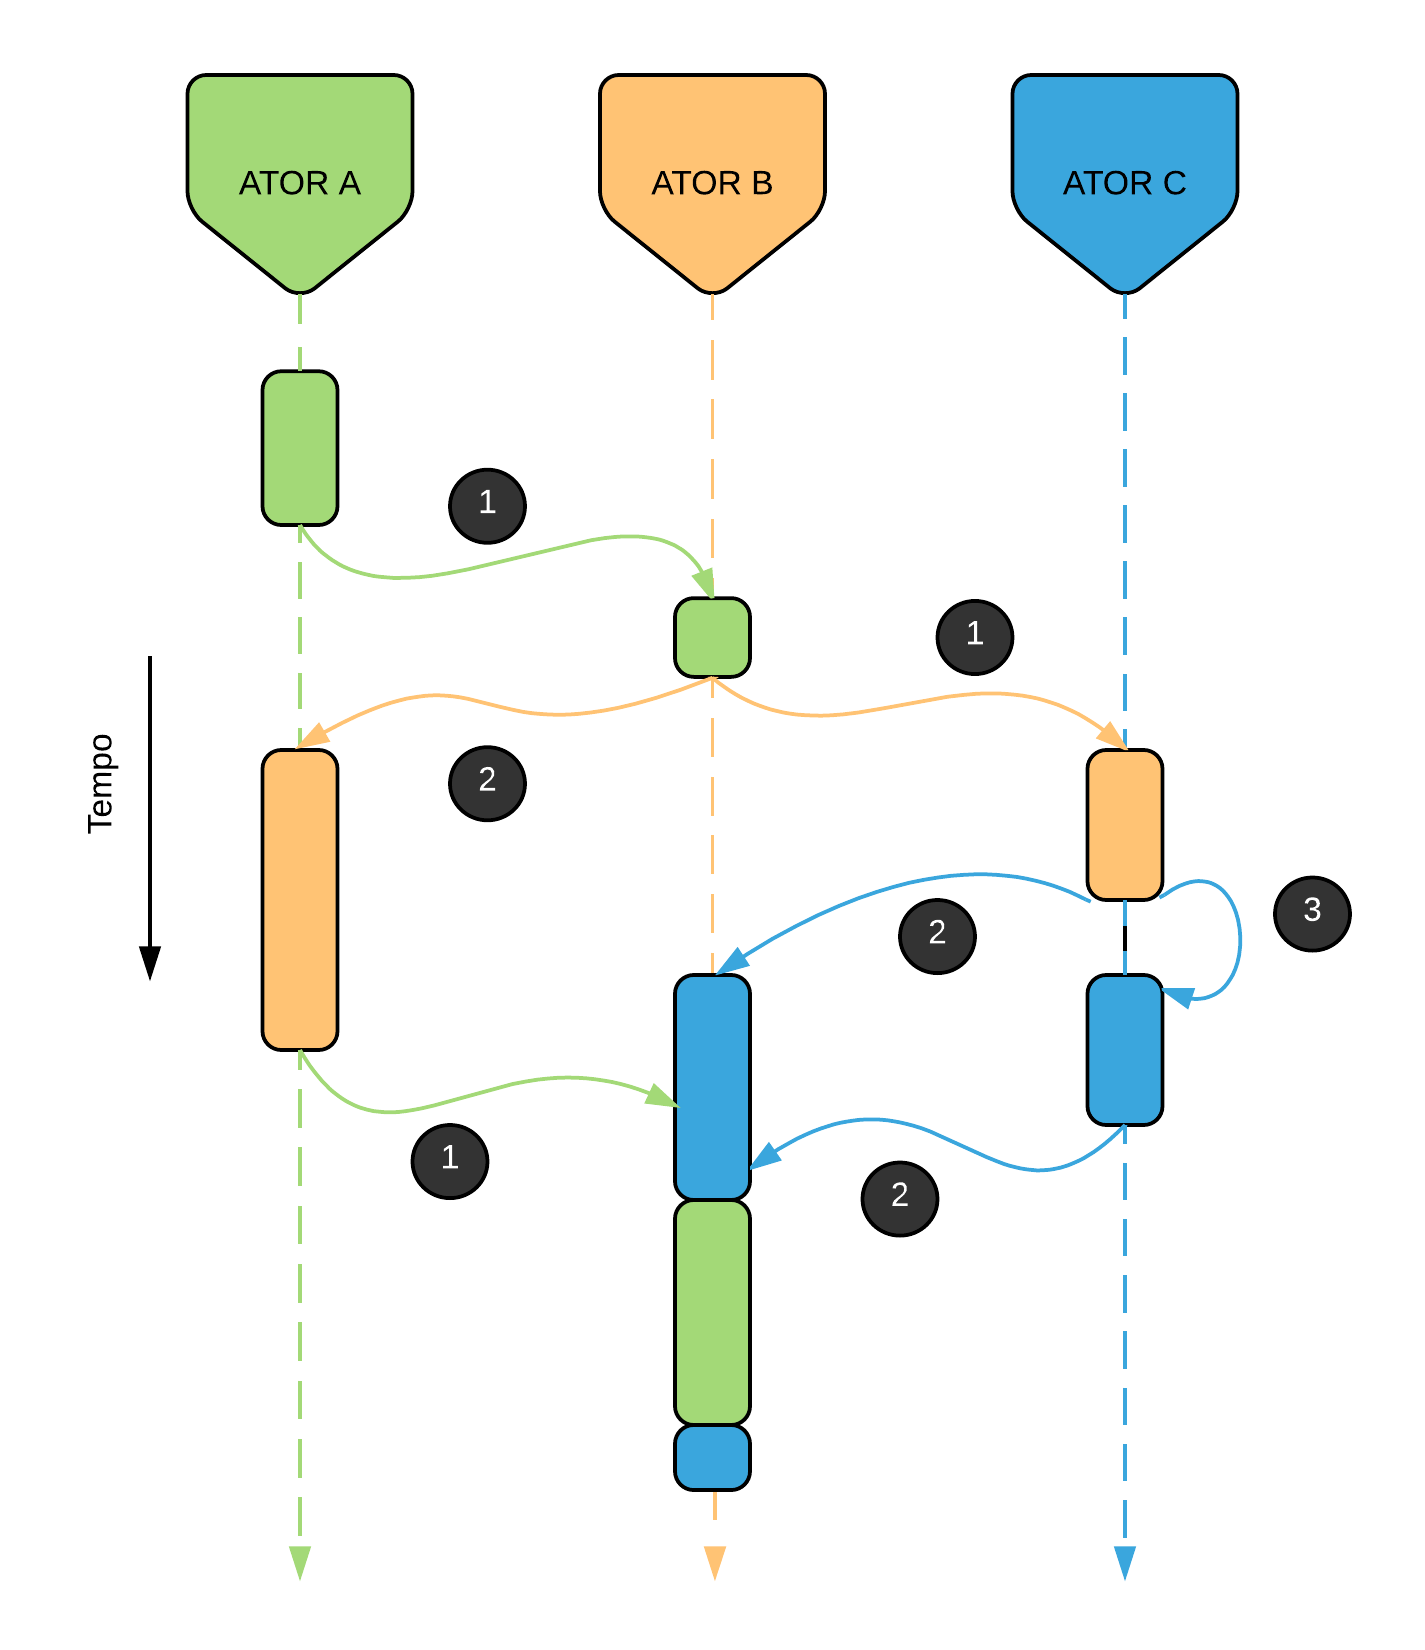
\includegraphics[width=0.9\linewidth]{fig/actormsg}
    \caption{Mensagens no \textit{framework} de atores em LabVIEW: (1) atores podem mandar mensagens para seus filhos; (2) atores podem mandar mensagem para os seus pais; (3) atores podem mandar mensagem para si mesmos}
    \label{fig:actormsg}
\end{figure}

Um ponto curioso do \textit{framework} é o suporte às mensagens síncronas entre atores \citep{smithAF}, funcionalidade que cria um compartilhamento de estado e rompe com a proposta do modelo.

% https://books.google.com.br/books?hl=en&lr=&id=s4AR6y1cp5EC&oi=fnd&pg=PA159&dq=actor+model&ots=x-POw6gaOc&sig=AhvfbolBXNsxexNgxGVpMoqShKs#v=onepage&q=actor%20model&f=false
% https://arxiv.org/ftp/arxiv/papers/1008/1008.1459.pdf
% http://berb.github.io/diploma-thesis/original/054_actors.html

\begin{comment}

O que eu quero falar na revisão?
Esta revisão bibliográfica pretende atingir dois objetivos: a revisão do estado da arte em teste de  placas eletrônicas, e também dos fundamentos do uso de programação concorrente, foco deste trabalho


Definir teste e diagnóstico.
Teste é o procedimento de checagem realizado para garantir a qualidade, desempenho, e confiabilidade de algo antes de ser colocado em uso
Diagnóstico é a identificação de uma causa raiz de um problema pela examinação de seus sintomas.
Metricas

O que eu quero falar na revisão?
Esta revisão bibliográfica pretende atingir dois objetivos: a revisão do estado da arte em placas eletrônicas, e também dos fundamentos do uso de programação concorrente, foco deste trabalho
\end{comment}